\documentclass[10pt,a4paper]{article}
\usepackage[utf8]{inputenc}
\usepackage[T1]{fontenc}
\usepackage{graphicx}
\usepackage{float}
\usepackage{amsmath}
\usepackage{amsfonts}
\usepackage{amsthm}
\theoremstyle{definition}
\newtheorem{definition}{Definition}[part]
\newtheorem{subdefinition}{Definition}[definition]
\theoremstyle{plain}
\newtheorem{example}{Example}[definition]

\title{Machine Learning 2023}
\author{David Graf}
\date{\today}
\begin{document}
\maketitle
\part{Preliminaries}
\begin{definition}[$\sigma$-Algebra]
	Let S be a non-empty set. A family of sets $F \subset P(S)$ is called a $\sigma$-Algebra on S, if the following conditions hold:
	\begin{itemize}
		\item $S \in F$
		\item From $ A \in F$, it follows that $A^c = S \setminus A \ \ \in F$
		\item From $ A_i \in F$, $i \in \mathbb{N}$, it follows that $$
			\bigcup_{i=1}^{\infty} A_i \  \in F$$
	\end{itemize}
\end{definition}

\paragraph{Remark:} Any subset $F \in P(S)$ is called a family of sets.\\

Smallest $\sigma$-Algebra over S: $\{\emptyset, S\}$\\

$\sigma$-Algebra generated by A: if $A \in S$, then,$$
\sigma(A) = \{\emptyset, A, A^c, S\}
$$
is the $\sigma$-Algebra generated by A.\\

\begin{definition}[Generator]
	\label{generator}
	Given $\varepsilon \ \subset \ P(S)$ (a family of sets) and $\Sigma$ denoting the set of \underline{all} $\sigma$-Algebras that contain $\varepsilon$, we call\\
	$$\sigma(\varepsilon) = \bigcap_{F \in S} F$$
	the $\sigma$-Algebra generated by $\varepsilon$. Further, if it holds that for a $\sigma$-Algebra A\\
	$$\sigma(\varepsilon) = A$$
	we call $\varepsilon$ the \underline{\textbf{generator}} of A.	
\end{definition}

\begin{example}
$\varepsilon = \big\{ \{1\} \big\}$ and $S = \big\{ \{1, 2, 3\} \big\}$:\\
$\sigma(\varepsilon) = \sigma(\big\{ \{1\} \big\}) = \big\{\emptyset, \{1\}, \{2, 3\}, \{1, 2, 3\} \big\} $
\end{example}

\begin{definition}[Topological Space]
A topological space is a tuple (X, $\tau$) with X a set and $\tau$ a collection of subsets of X such that
	\begin{enumerate}
		\item $\emptyset, X \in \tau$
		\item closed under \underline{union}, i.e.,\\
		 $$ \{ U_i \}_{i \in I} \subseteq \tau \implies \bigcup_{i \in I} U_i \in \tau$$
		\item closed under \underline{finite intersection}, i.e., \\
			$$\{ U_i \}_{i = 1}^n \subseteq \tau \implies \bigcap_{i = 1}^{n} U_i \in \tau$$
	\end{enumerate}
\textbf{Remark:} The elements of $\tau$ are called \underline{open sets}!
\end{definition}

\begin{definition}[Borel $\sigma$-Algebra]
	Given a topological space (S, O) with O denoting the system of open sets, then we call
	$$B(s) := \sigma(O)$$
	the \underline{Borel $\sigma$-Algebra} over S. Its elements are called Borel sets.\\
	$ S = \mathbb{R}^n$, we write $\mathbb{B}^n := \mathbb{B}(\mathbb{R}^n)$\\
	
	Each of the following systems of sets are generators for $\mathbb{B}(\mathbb{R}^n) = \mathbb{B}^n$:
	\begin{enumerate}
		\item $\{U \subset \mathbb{R}^n$: U open $\}$
		\item $\{A \subset \mathbb{R}^n$: A closed$\}$
		\item $\big\{ ]a,b ] : a, b\in \mathbb{R}^n,\ a\subseteq b \big\} $
	\end{enumerate}
\end{definition}

\paragraph{Convention:} We extend $\mathbb{R}$ by symbols "$-\infty$" and "$+\infty$" as\\
	$$ \overline{\mathbb{R}} = \mathbb{R} \cup \{+\infty, -\infty\} $$
	$$ \overline{\mathbb{B}} = \sigma(\mathbb{B} \cup \{+\infty\} \cup \{-\infty\} )$$

\begin{definition}[Measurable space]
	\label{Measurable_Space}
	If F is a $\sigma$-Algebra over S, we call (S,F) a \underline{measurable space}. 
\end{definition}

\begin{subdefinition}[Measurable maps/functions]
	Given $(S_1, F_1)$ and $(S_2, F_2)$, we call
	$$f: S_1 \rightarrow S_2$$
	a measurable function ($F_1$-$F_2$-measurable) if
	 $$\forall E \in F_2: f^{-1}(E) \subset F_1$$
\end{subdefinition}

\begin{example}
$1_A : S \rightarrow \{0, 1\}$ indicator function of set $A \subset S$
$$w \mapsto 1_A(w) \begin{cases}
	1, & \text{if}\ w \in A \\
	0, & else
\end{cases}$$
Consider $1_A$ as a function to $\mathbb{R}$.
\begin{itemize}
	\item if $\beta \leq 0$, then $\{w: 1_A(w)<\beta\} = \emptyset$
	\item if $\beta > 1$, then $\{w: 1_A(w)<\beta\} = S$
	\item if $0 < \beta \leq 1$, then $\{w: 1_A(w)<\beta\} = S \setminus A$
\end{itemize}
$\implies 1_A$ is measurable if $A \in F$ (S, F)
\end{example}

\begin{definition}[Measure]
	\label{measure}
	Let (S,F) be a measurable space. A function
	$$\mu: F \rightarrow \bar{\mathbb{R}}$$
	is called a \underline{measure} if the following conditions hold:
	\begin{enumerate}
		\item $\mu(\emptyset) = 0$
		\item $\mu(A) \geq 0$ for all $A \in F$
		\item  for every sequence of $(A_n)_{n \in \mathbb{N}}$ of disjoint sets from F, we have 
			\begin{equation}
				\tag{$\sigma\text{-Additivity}$}
				\mu (\bigcup_{i = 1}^{\infty} A_i) = \sum_{i = 1}^{\infty} \mu(A_i)
			\end{equation} 
	\end{enumerate}
\end{definition}

\begin{subdefinition}[Measure space]
	given a measurable space (S, F) and a measure $\mu: F \rightarrow \bar{\mathbb{R}}$, we call
	$$(S, F, \mu)$$
	a \underline{measure space}.
\end{subdefinition}

\paragraph{Some important properties of measure spaces:} let A, B, $A_n \in F$, $n \in \mathbb{N}$. Then
\begin{enumerate}
	\item if A and B are disjoint, then $\mu(A \cup B) = \mu(A) + \mu(B)$
	\item if $A \subset B$ and $\mu(A) < \infty$, then
	$$ \mu(B\setminus A) = \mu(B)-\mu(A)$$
	\item if $A \subset B$, then
	 $$\mu(A) \leq \mu(B)$$
	\item \begin{equation}
		\tag{$\sigma\text{-sub-Additivity}$}
		\mu (\bigcup_{i = 1}^{\infty} A_i) \leq \sum_{i = 1}^{\infty} \mu(A_i)
	\end{equation}
\end{enumerate}

\begin{definition}[Probability Space]
	Given ($\mathcal{S}$, $\mathcal{F}$, $\mathcal{D}$) a measure space, with 
	$$\mathcal{D}(\mathcal{S}) = 1$$
	then we call D a \underline{probability measure} and ($\mathcal{S}$, $\mathcal{F}$, $\mathcal{D}$) a \underline{probability space}.
	(A set S, a sigma algebra F on that set, and a measure D that assigns to every element of F a probability (a number between 0 and 1)
\end{definition}
\paragraph{Remark:} A possibility to construct, based on a measure space $(S_1, F_1, \mu)$ and a measurable function f from $S_1$ to $S_2$ (with $(S_2, F_2)$), another measure space $(S_2, F_2, \mu_F)$:
\begin{eqnarray*}
	\mu_F: & F_2 \rightarrow [0, \infty] \\
	 B\mapsto & \mu_f(B) := \mu(f^{-1} (B))
\end{eqnarray*}  
\begin{definition}[Random variable]
	If $(S_1, F_1, D)$ is a probability space and $(S_2, F_2)$ a measurable space, then
	$$X: S_1 \rightarrow S_2$$
	is called a \underline{random variable}. \\
	For $S_2 = \mathbb{R}$, we call X a real random variable. The \underline{push-forward measure} $\mathbb{P}_x$ on $(S_2, F_2)$ is also a probability measure.
	$$\underbrace{\mathbb{P}_x(S_2)}_{\text{"distribution" of X}} = D(X^{-1}(S_2)) = D(S_1) = 1$$
\end{definition}
\paragraph{Conventions:}
\begin{eqnarray*}
\{ X \in A \} = \{w \in S: X(w) \in A \}\\
\{X = c\} = \{w \in S: X(w) = c\}\\
\mathbb{P}_x(A) = D\big(\{w \in S: X(w) \in A\}\big)\\
\mathbb{P}_x(\{c\}) = D\big(\{w \in S: X(w) = c\}\big)\\	
\end{eqnarray*}

\paragraph{Idea of Riemann Integral}:

\begin{figure}[H]
	\centering
	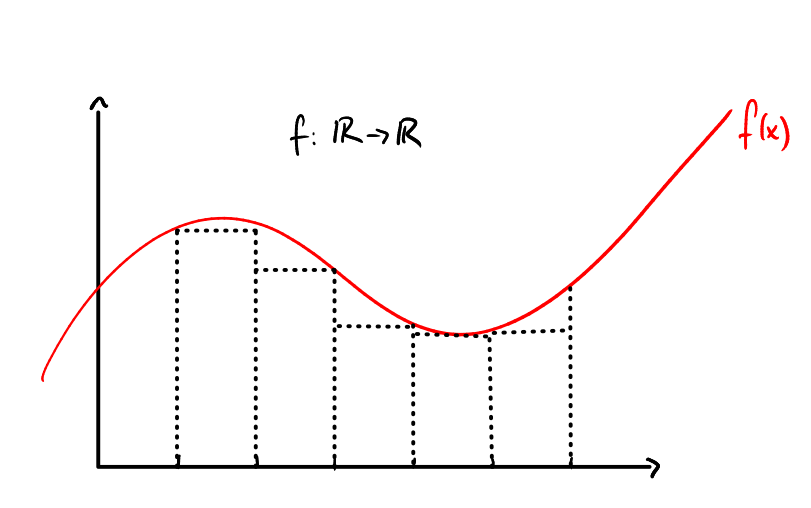
\includegraphics[width=0.7\linewidth]{riemann_idea}
	\caption{Graphical Representation of Riemann Integration}
	\label{fig:riemannidea}
\end{figure}
Problems:
\begin{figure}[H]
\minipage{0.62\textwidth}
\begin{itemize}
	\item Difficult to extend to higher dimensions (3-d?)
	\item Reliance on continuity (what about discontinuous functions?)
	\item ...
\end{itemize}
\endminipage\hfill
\minipage{0.32\textwidth}
	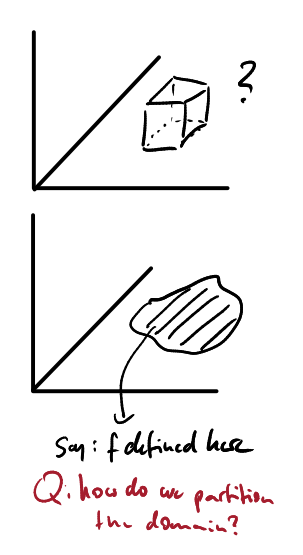
\includegraphics[width=.5\linewidth]{riemann_problems}
	\label{fig:riemann_problems}
\endminipage\hfill
\end{figure}
\paragraph{Idea of Lebesque-Integration} The key idea is to partition the range of a function $f: S \to \mathbb{R}$ in intervals, to get an approximation by "elementary" functions.
\begin{figure}[H]
	\centering
	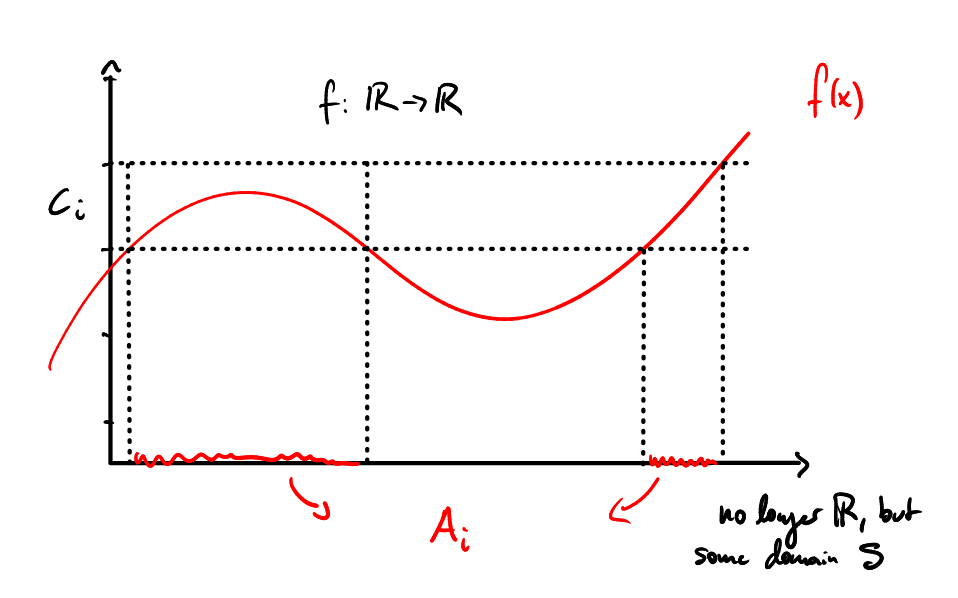
\includegraphics[width=0.7\linewidth]{lebesque_idea}
	\caption{Graphical Representation of Lebesque Integration}
	\label{fig:lebesqueidea}
\end{figure}
We need a way to measure $A_i$. If we can do that, we can write:
$$ c_{i} \ . \ \underbrace{\mu(A_i)}_{\text{measure}}$$
... this will allow us to eventually write
$$ \sum_{i} c_i \mu(A_i) \ \text{  \underline{or}  }  \int_{S}f d\mu$$

\paragraph{In a little bit more detail} In particular, lets look at case of "simple" functions. Say, we have (S, F, $\mu$), $\mu: F \to [0, \infty]$.

\begin{figure}[H]
	\centering
	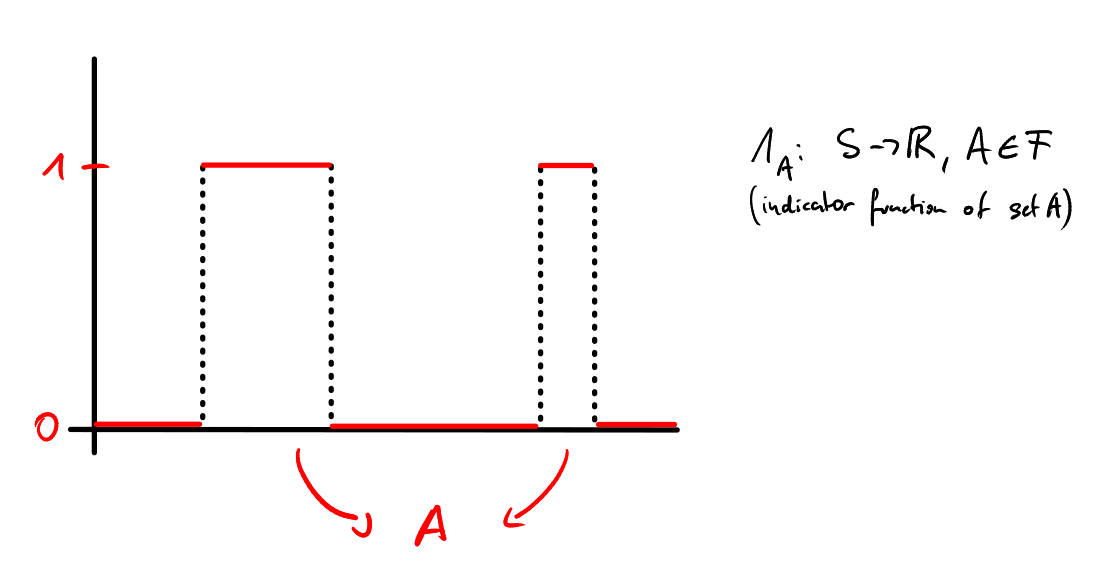
\includegraphics[width=0.7\linewidth]{leb_detail}
	\caption{Illustration of indicator function of A}
	\label{fig:lebdetail}
\end{figure}
Any reasonable integration of $1_A$ should return $\mu_A$.
$$ \underbrace{I(1_A)}_{\text{integral}} = \mu_A$$
What is a "simple" function? $ f(x) = \sum_{i=1}^{n} c_i \cdot 1_{A_{i}} \cdot (x), \ \ A_i \in F, c_i \in \mathbb{R}$\\
\begin{figure}[H]
	\centering
	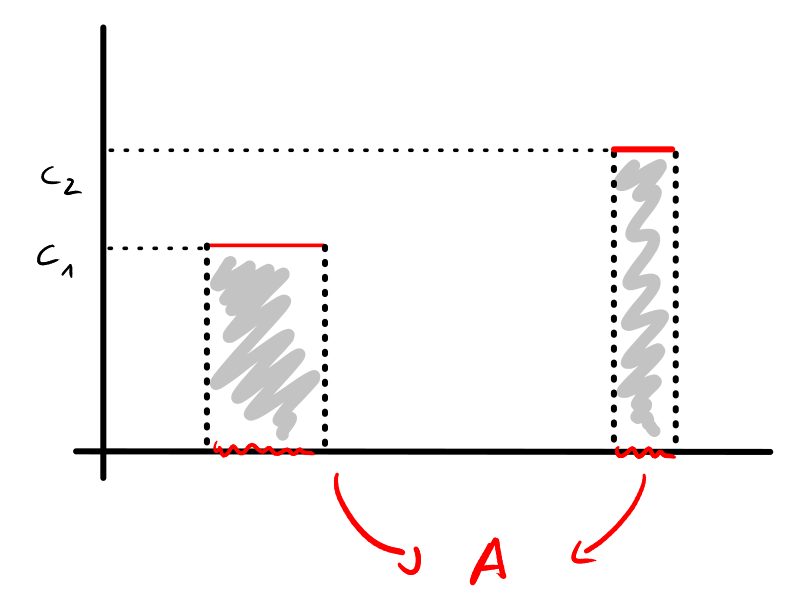
\includegraphics[width=0.5\linewidth]{simple_leb}
	\caption{Graphical Representation of simple lebesque integrable function}
	\label{fig:simplefun}
\end{figure}


We can define the interval of f via
$$ I(f) = \sum_{i = 1}^{n} c_i \cdot \mu(A_i)$$
Problem: $\mu: F \to [0, \infty], c_i \in \mathbb{R} \implies$ so, we could get something like $10 \cdot \infty - 3 \cdot \infty$.\newline

Solution: $\{f: S \to \mathbb{R}\ \big| \ \text{f is "simple" and } f \geq 0\} = T^+
$\\

For $f \in T^+$, we have a representation of f as
$$f(x) = \sum_{i=1}^{n} c_i \cdot 1_{A_i}(x) \text{ with } c_i \geq 0$$
and we define the lebesque integral as 
$$ I(f) = \sum_{i=1}^{n} c_i \cdot \mu_{A_i} \text{ or } \int f d_{\mu} \text{ , or } \int f(x) d_{\mu}(x)$$

\paragraph{Properties} 
\begin{enumerate}
	\item For f, g $\in T^+$, and $\alpha, \beta \geq 0$ 
	
	\begin{equation}
		\tag{\textbf{Linearity}}
	 	\int (\alpha f + \beta g)d_\mu = \alpha \cdot \int fd_\mu + \beta \int gd_\mu
	 \end{equation}
	\item  if $f, g \in T^+$ and $ f \leq g$, it follows that 
	\begin{equation}
		\tag{\textbf{Monotonicity}}
		\int fd_\mu \leq \int gd_\mu
	\end{equation}
\end{enumerate}
This construction extends to all measurable functions $f: S\to \mathbb{R}\ $ !

\begin{definition}[Expected value of a random variable]
	Given a probability space (S, F, D) and a (quasi-integrable) real random variable $X: S \to R$, then
	$$ \mathbb{E}[X] = \int XdD$$
	is the \underline{expected value} of X.
\end{definition}
\paragraph{Properties}
\begin{enumerate}
	\item if $X\geq 0$, then $\mathbb{E}[X] \geq 0$
	\item $\mathbb{E}[X+Y] = \mathbb{E}[X] + \mathbb{E}[Y]$ for random variables $X$ and $Y$
\end{enumerate}
\begin{definition}[Markov Inequality]
	Given a probability space (S, F, D) and a non-negative ($\geq 0$) random variable X, we have for $ a > 0$ 
	$$ \mathbb{P}[X\geq a] \leq \frac{\mathbb{E}[X]}{a}$$
	$$ \Bigg( \mathbb{P}[X\geq a] = D\Big(\{\omega \in S: X(\omega) \geq a \} \Big)\Bigg)$$
\end{definition}
\begin{proof}
	We define $\Phi: S \to \mathbb{R}$ with
	$$ \Phi(x) = \begin{cases}
		a, & \text{if}\ X \leq a \\
		0, & \text{if}\ X < a
	\end{cases} $$
	$\implies O \leq \Phi(X) \leq X(x)$. Hence, by monotonicity, we have
	\begin{equation*}
	\begin{split}
		\int XdD &\geq \int \Phi dD\\
				&= a\cdot D\big( \{\omega \in S: X(\omega) \geq a\}\big)
	\end{split}		
	\end{equation*}
	
	Divide by $a>0$
	$$ \implies \frac{1}{a} \cdot \int XdD \ \geq D\big( \{\omega \in S: X(\omega \geq a) \} \big) = \mathbb{P}[X\geq a]$$
	Since $\int XdD$ is $\mathbb{E}[X]$, we get $\mathbb{P}[X\geq a]\leq \frac{\mathbb{E}[X]}{a}$
\end{proof}
%
%\part{Actual ML lecture content}
%Recap of our setup:
%\begin{enumerate}
%	\item DOMAIN set X; we call $x\in X$ an instance
%	\item LABEL set Y; e.g. $Y = \{0, 1\}$ (for a binary problem)
%	\item TRAINING set $S = \big((x_1, y_1), ..., (x_m, y_m)\big)$  with $x_i \in X, y_i \in Y$
%	\item a LEARNER that receives S and outputs 
%	$$ h: X \to Y$$
%	which we call a hypothesis
%\end{enumerate}
%Assumption: for now, we assume $x_i$'s are drawn iid from some probability measure D over the domain and labelled by some function $f: X \to Y$:
%$$ x_i \underbrace{ \sim }_{\text{\scriptsize"drawn from"}} D,\ y_i = f(x_i)$$
\end{document}